%---------------------------------------------------------------------------------------------------
% Einstellungen
% (gelten nur in Zusammenarbeit mit pdflatex)
%---------------------------------------------------------------------------------------------------
\documentclass[
  pagesize, % flexible Auswahl des Papierformats
  a4paper, % DIN A4
  oneside, % einseitiger Druck
  BCOR5mm, % Bindungskorrektur
  headsepline, % Strich unter der Kopfzeile
  11pt, % 11pt Schriftgröße
  halfparskip, % Europäischer Satz: Abstand zwischen Absätzen
  abstracton, % Spezielle Formatierung, die erlaubt, dass die Zusammenfassung vor dem Inhaltsverzeichnis steht
  %draft, % Es handelt sich um eine Vorabversion
  final, % Es handelt sich um die endgültige Version
  liststotoc, % Tabellen- und Abbildungsverzeichnis im Inhaltsverzeichnis
  idxtotoc, % Index im Inhaltsverzeichnis
  bibtotoc,                                            % Literaturverzeichnis im Inhaltsverzeichnis
]{scrartcl}                                            % KOMA-Scriptklasse Report

%---------------------------------------------------------------------------------------------------
\usepackage[english,ngerman]{babel}                    % deutsche Trennmuster
\usepackage[T1]{fontenc}                               % EC-Schriften, Trennstellen nach Umlauten
\usepackage[utf8x]{inputenc}                          % direkte Umlauteingabe (ä statt "a)
                                                       % latin1/latin9 für unixoide Systeme
                                                       % (latin1 ist auch unter Win verwendbar)
                                                       % ansinew für Windows
                                                       % applemac Macs
                                                       % cp850 OS/2
\usepackage{times}                                     % Schriften Paket
\usepackage{array,ragged2e}                            % Wichtig für Abstandsformatierung

%---------------------------------------------------------------------------------------------------
\usepackage{cmbright}                                  % serifenlose Schrift als Standard
                                                       % + alle für TeX benötigten mathematischen
                                                       %   Schriften einschließlich der AMS-Symbole
\usepackage[scaled=.90]{helvet}                        % skalierte Helvetica als \sfdefault
\usepackage{courier}                                   % Courier als \ttdefault

%---------------------------------------------------------------------------------------------------
\usepackage[automark]{scrpage2}                        % Anpassung der Kopf- und Fußzeilen
\usepackage{xspace}                                    % Korrekter Leerraum nach Befehlsdefinitionen
\usepackage{setspace}                                  % Dieses Package brauchen wir für den anderthalbzeiligen Abstand.
\usepackage[numbers]{natbib}                           % Neuimplementierung des \cite-Kommandos
%\usepackage{bibgerm}                                  % Deutsche Bezeichnungen (deprecated)
\usepackage[german]{babelbib}                          % Deutsche Bezeichnungen
\usepackage[absolute, overlay]{textpos}                % placing boxes at absolute positions
\usepackage[final]{pdfpages}                           % include pages of external PDF documents
\usepackage{tabularx}                                  % Spaltenbreite bis zur Seitenbreite dehnen
\usepackage{makeidx}                                   % Paket zur Erstellung eines Stichwortverzeichnisses
\makeindex                                             % Automatische Erstellung des Stichwortverzeichnis
\usepackage[intoc,german,prefix]{nomencl}

% \usepackage{footnote} % Ermöglicht Fußnoten in gleitenden Umgebungen
% \usepackage{capt-of} % Ermöglicht Beschriftungen beliebiger Objekte

\makenomenclature

%---------------------------------------------------------------------------------------------------
 \usepackage{graphicx}                                 % Zur Einbindung von PDF-Bildern
 \usepackage[colorlinks,                               % Einstellen und Laden des Hyperref-Pakets
  pdftex,
  bookmarks,
  bookmarksopen=false,
  bookmarksnumbered,
  citecolor=blue,
  linkcolor=blue,
  urlcolor=blue,
  filecolor=blue,
  linktocpage,
  pdfstartview=Fit,                                  % startet mit Ganzseitenanzeige
  pdfsubject={Erweiterung des Routing-Atlas},
  pdftitle={Erweiterung des Routing-Atlas - Ausarbeitung: Seminar)},
  pdfauthor={Andreas Krohn}]{hyperref}
% \pdfcompresslevel=9
%\usepackage{wrapfig}

%---------------------------------------------------------------------------------------------------
% Inhaltsverzeichnis und Abschnittnummerierung
%---------------------------------------------------------------------------------------------------
\setcounter{secnumdepth}{2}   % Ich habe recht kurze Kapitel. Die sollen nicht durchnummeriert sein.
\setcounter{tocdepth}{2}

%---------------------------------------------------------------------------------------------------
% Abbildungsverzeichnis
%---------------------------------------------------------------------------------------------------
\graphicspath{{graphics/}}

%---------------------------------------------------------------------------------------------------
% Kopf- und Fußzeilen
%---------------------------------------------------------------------------------------------------
\pagestyle{scrheadings}
\clearscrheadings
\clearscrplain
\clearscrheadfoot
\ohead{\pagemark}
\ihead{\headmark}

%---------------------------------------------------------------------------------------------------
% Neue Befehle
%---------------------------------------------------------------------------------------------------
%---------------------------------------------------------------------------------------------------
% Neue Befehle
%---------------------------------------------------------------------------------------------------

%---------------------------------------------------------------------------------------------------
% Umbenennen des Symbolverzeichnisses
%---------------------------------------------------------------------------------------------------
\renewcommand{\nomname}{Glossar}				% Das Symbolverzeichnis heisst nun "Glossar"
\renewcommand{\nomlabel}[1]{						% Die zu erklärenden Begriffe sind nun fett hervorgehoben
	\hfil \textbf{#1} \hfil
}

%---------------------------------------------------------------------------------------------------
% Ein paar ganz nützliche Befehle von Lars Mählmann
%---------------------------------------------------------------------------------------------------
%für Kommentare
\newcommand{\colb}{\color{green}}
\newcommand{\colbl}{\color{black}}

%---------------------------------------------------------------------------------------------------
% Befehle zum Erstellen des Index
% \addIndexEntry{Eintrag in den Index}
% \addSubIndexEntry{Eintrag in den Index}{Eintrag des übergeordneten Eintrags}
%---------------------------------------------------------------------------------------------------
\newcommand{\addIndexEntry}[1]{#1\index{#1}}
\newcommand{\addSubIndexEntry}[2]{#1\index{#2!#1}}

%---------------------------------------------------------------------------------------------------
% LaTeX in eigenem Font
%---------------------------------------------------------------------------------------------------
\newcommand{\myLatex}{
	{\rmfamily\LaTeX\xspace}
}

%---------------------------------------------------------------------------------------------------
% Befehl zum Erstellen und Hervorheben eines Zitats
% Parameter:
% 1. Zitat
% 2. Author
% 3. Quelle
%---------------------------------------------------------------------------------------------------
\newcommand{\myCitation}[3]{
	\begin{flushright}
	\begin{minipage}{.4\linewidth}
		\footnotesize\rmfamily\itshape
		#1 \\
		\RaggedLeft #2 \\
		#3
	\end{minipage}
	\end{flushright}
	\nobreakspace
}

%---------------------------------------------------------------------------------------------------
% Erstellung von Deckblatt (Seite 1) und Titelblatt (Seite 2)
%---------------------------------------------------------------------------------------------------
\newcommand{\createCoverAndTitlePage}[8]{
	\createCover{#1}{#2}{#3}
	\createTitlePage{#1}{#2}{#3}{#4}{#5}{#6}{#7}{#8}
}

%---------------------------------------------------------------------------------------------------
% Erstellung von Deckblatt (Seite 1)
% Anwendung:
% \createCover{Art der Arbeit}{Autor}{Titel}
%---------------------------------------------------------------------------------------------------
\newcommand{\createCover}[3]{
	\thispagestyle{empty}
	\begin{titlepage}

	\setlength{\TPHorizModule}{1mm}
	\setlength{\TPVertModule}{1mm}
	\textblockorigin{0mm}{0mm} % start everything near the top-left corner

	% Art der Arbeit
	\begin{textblock}{111}(83,115)
		\begin{minipage}[c][1,78cm][c]{11,09cm}
  		\fontsize{22pt}{20pt}
  		\selectfont
  		\begin{center}
  		#1
  		\end{center}
		\end{minipage}
	\end{textblock}

	% Name & Titel
	\begin{textblock}{111}(83,131)
		\begin{minipage}[c][4,81cm][t]{11,09cm}
		\linespread{1.2}
    \fontsize{16pt}{14pt}
    \selectfont
    \begin{center}
    #2 \\ \medskip
    #3
    \end{center}
    \end{minipage}
	\end{textblock}
	% Infos zur Arbeit und zum Fachbereich
	\begin{textblock}{186}(22,264)
  	\begin{minipage}[t][5,72cm][l]{17,57cm}
    	\fontsize{12pt}{12pt}
    	\selectfont
			{\em Fakultät Technik und Informatik \hfill Faculty of Engineering and Computer Science}\\
			{\em Department Informatik \hfill Department of Computer Science}
  	\end{minipage}
	\end{textblock}
	\newpage
	\end{titlepage}
%---------------------------------------------------------------------------------------------------
% Wichtig! Entsprechendes Auskommentieren!
%---------------------------------------------------------------------------------------------------
	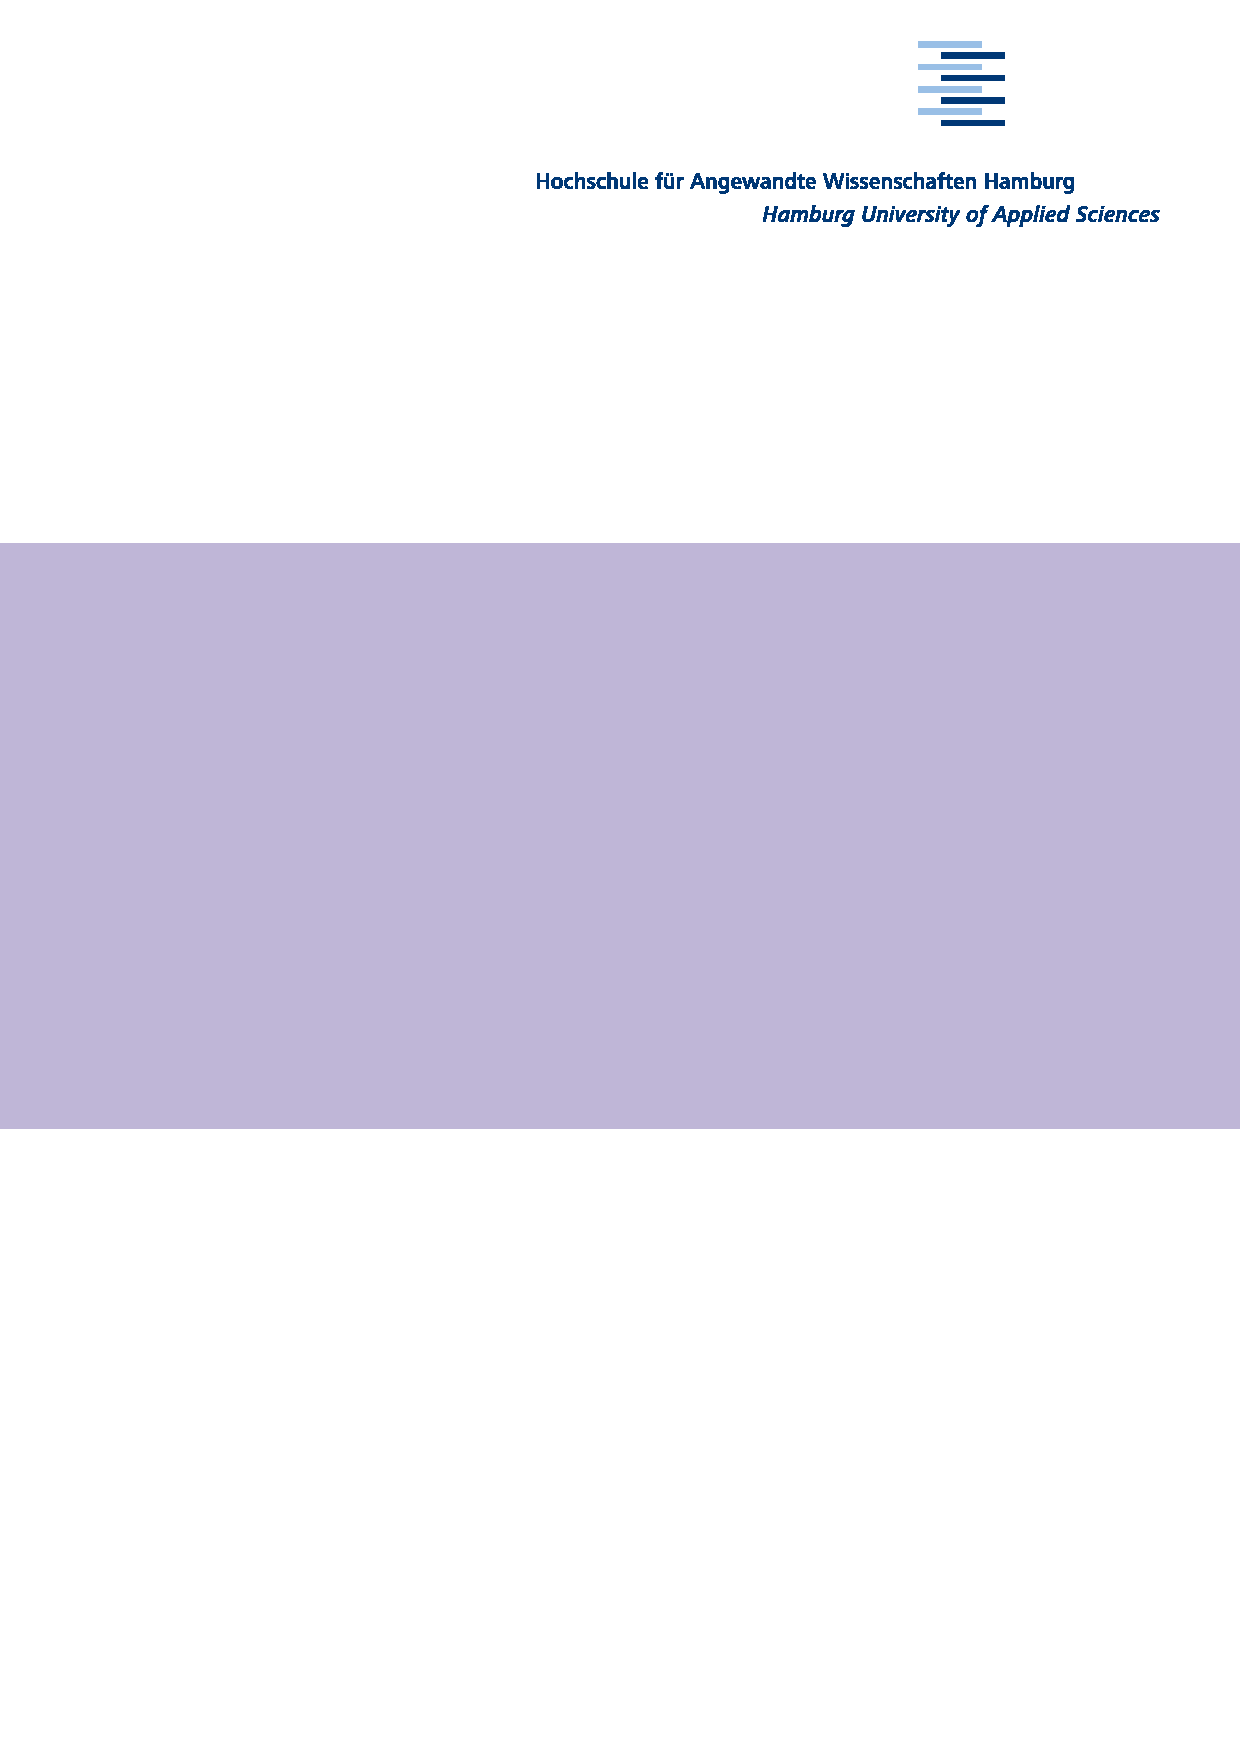
\includepdf{pdf/titel}           				% zum Ausdruck auf blanko Papier
  %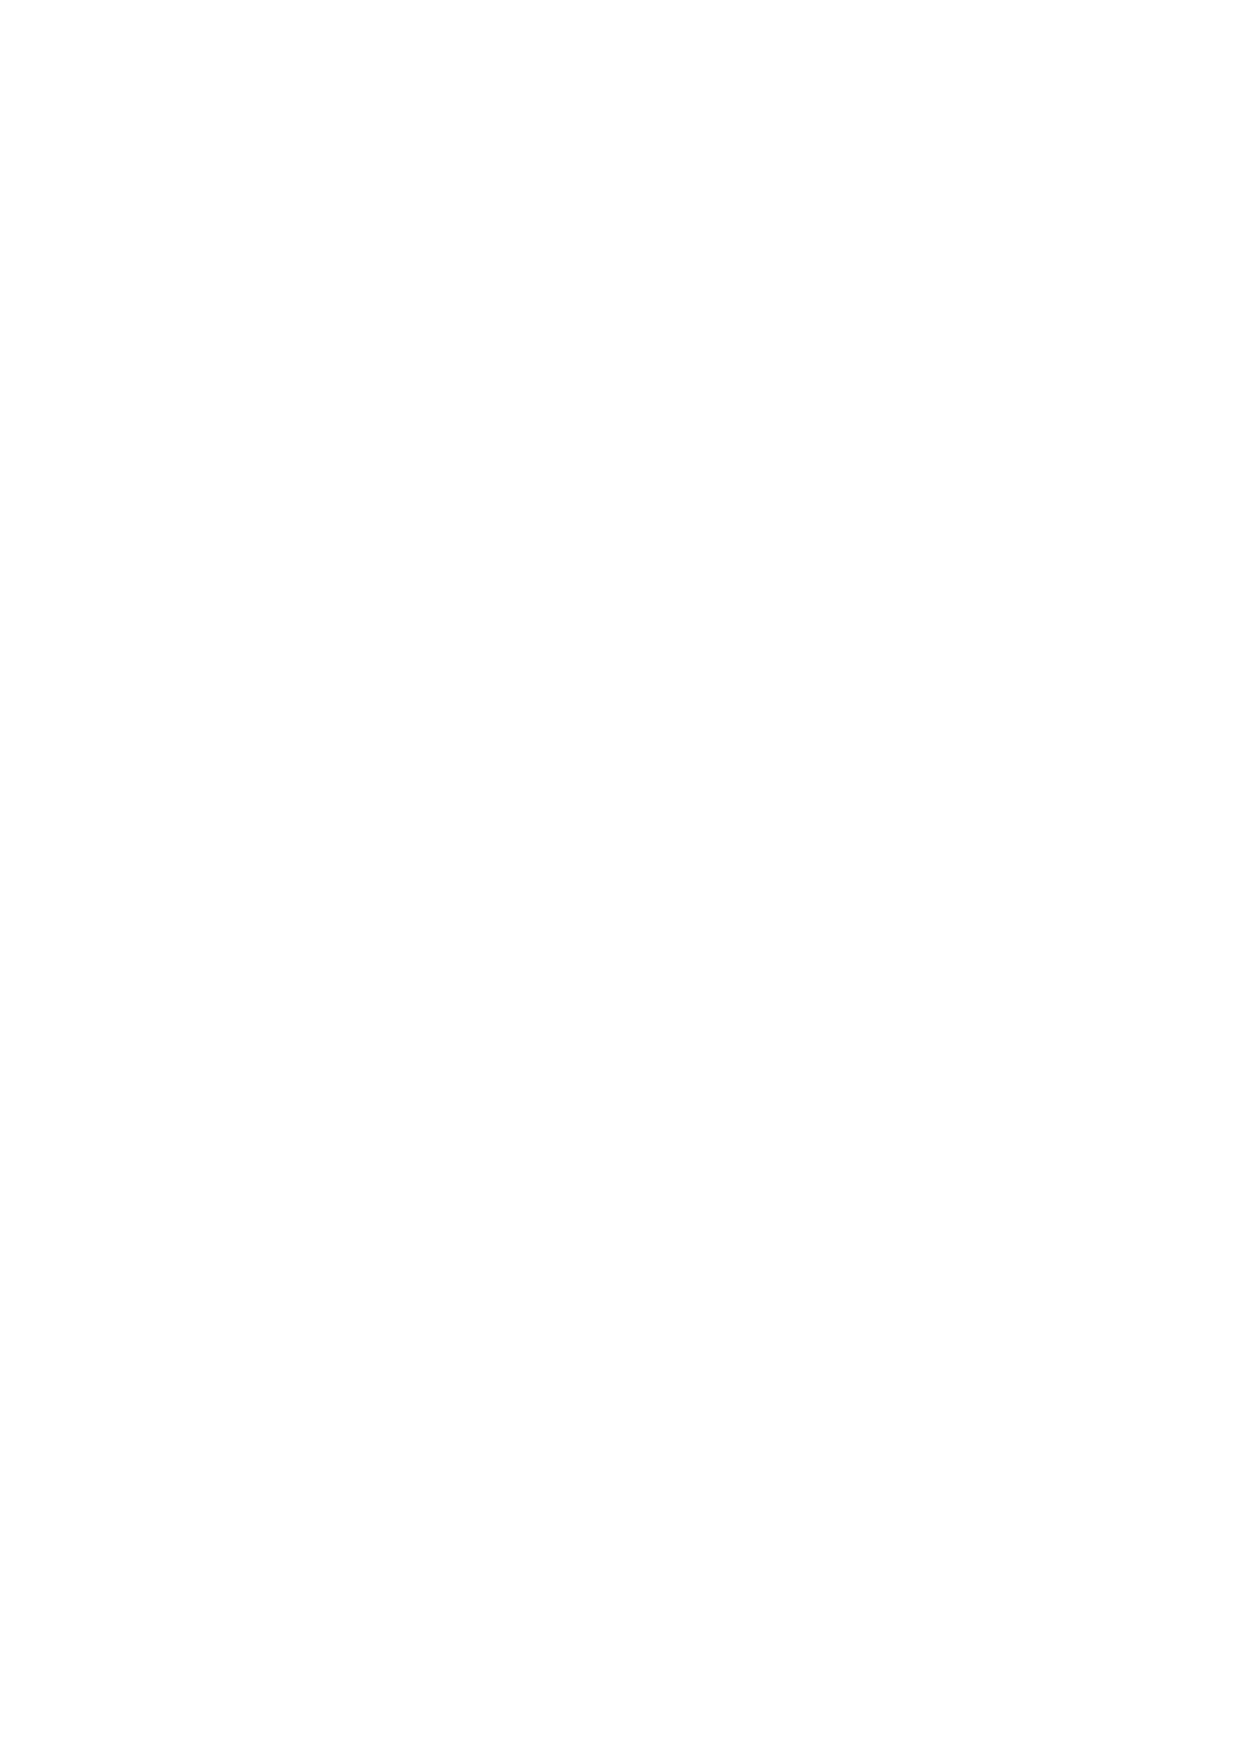
\includepdf{pdf/titel_leer}           	% zum Ausdruck auf die Pappe
}

%---------------------------------------------------------------------------------------------------
% Erstellung von Titelblatt (Seite 2)
% Anwendung:
% \createTitlePage{Art der Arbeit}{Author}{Titel}{Studiengang}{Erstprüfer}{Zweitprüfer}
%---------------------------------------------------------------------------------------------------
\newcommand{\createTitlePage}[7]{
	\thispagestyle{empty}

	\setlength{\TPHorizModule}{1mm}
	\setlength{\TPVertModule}{\TPHorizModule}
	\textblockorigin{0mm}{0mm} % start everything near the top-left corner

	% Name & Titel
	\begin{textblock}{130}(40,63)
		\begin{minipage}[c][5,9cm][t]{13cm}
			\begin{center}
			\linespread{1.2}
			\fontsize{18pt}{18pt}
  		\selectfont
  		#2 \\ \medskip
  		\fontsize{16pt}{16pt}
  		#3
  		\end{center}
		\end{minipage}
	\end{textblock}

	% Infos zur Arbeit und zum Fachbereich
	\begin{textblock}{126}(32,214)
  	\begin{minipage}[t][5,72cm][l]{12,57cm}
    	\fontsize{12pt}{12pt}
    	\selectfont
    	#1 eingereicht im Rahmen der #1prüfung\\
    	im Studiengang #4\\
			am Department Informatik\\
			der Fakultät Technik und Informatik\\
			der Hochschule für Angewandte Wissenschaften Hamburg\\
			\\\
			\\\
			Betreuender Prüfer : #5\\
			Zweitgutachter : #6\\
			\\\
			Abgegeben am \today
  	\end{minipage}
	\end{textblock}
	\	% WICHTIG! Damit wird nach dem Titelblatt eine neue Seite angefangen! Sonst werden Titelblatt &
  	% Danksagung auf eine Seite gedruckt!
}

%---------------------------------------------------------------------------------------------------
% Versicherung über Selbstständigkeit
%---------------------------------------------------------------------------------------------------
\newcommand{\asurency}{
	\chapter*{Versicherung über Selbstständigkeit}
	\vfill
	Hiermit versichere ich, dass ich die vorliegende Arbeit im Sinne der Prü\-fungs\-ord\-nung nach \S 24(5) 		ohne fremde Hilfe selbstständig verfasst und nur die angegebenen Hilfsmittel benutzt habe.
	\vfill
	\begin{tabularx}{\linewidth}{X l X}
	Hamburg, \today	& \qquad \qquad \qquad	& \\
	\cline{1-1}
	\cline{3-3}
	Ort, Datum	& \qquad \qquad \qquad	& Unterschrift \\
	\end{tabularx}
	\vfill
	\vfill
	\vfill
}

%---------------------------------------------------------------------------------------------------
% Fügt ein Wort dem Index zu
%---------------------------------------------------------------------------------------------------
\newcommand{\toIndex}[1]{#1\index{#1}}

%---------------------------------------------------------------------------------------------------
% Dient zum Eintragen folgender Dinge in die Zusammenfassung (Abstract):
%	- Thema
% - Stichworte
% - Kurzfassung
% Benutzung wie folgt:
% \abstractentry{Titel}{Text}
%---------------------------------------------------------------------------------------------------
\newcommand{\abstractentry}[2]{
	\textbf{\large#1}\\
	\nobreakspace
	\begin{tabular}{lp{142mm}}
		\hspace*{7mm} & #2 \\
	\end{tabular}
	\vfill
}

%---------------------------------------------------------------------------------------------------
% Erstellt eine Defintion
% Anwendung: \definition{Die Definition}
%---------------------------------------------------------------------------------------------------
\newcommand{\definition}[1]{
\begin{tabular}[ht]{lp{135mm}}
	\textbf{Def.:} & #1 \\
\end{tabular}
}

%---------------------------------------------------------------------------------------------------
% Erstellt eine Widmung
% Anwendung: \dedication{Wem ist das Schriftstück gewidmet}
%---------------------------------------------------------------------------------------------------
\newcommand{\createDedication}[1]{
	\newpage
	\thispagestyle{empty}
	\begin{tabular}{lp{60mm}}
		\hspace*{100mm} & \itshape\rmfamily#1 \\
	\end{tabular}
	\vfill
}

%---------------------------------------------------------------------------------------------------
% Häufig verwendete Namen mit Literaturverweis und Indexeintrag
%--------------------------------------------------------------------------------------------------
\newcommand{\butrynowski}{Christian Butrynowski\index{Butrynowski, Christian} \citep{Butrynowski:2005}\xspace}
\newcommand{\luepke}{André Lüpke\index{Lüpke, André}\citep{Luepke:2004}\xspace}
\newcommand{\bresch}{Marco Bresch\index{Bresch, Marco} \citep{Bresch:2004}\xspace}


%---------------------------------------------------------------------------------------------------
% Die folgenden Befehle wurden aus der Vorlage von Michael Knop übernommen
%--------------------------------------------------------------------------------------------------
%---------------------------------------------------------------------------------------------------
% Ident
%---------------------------------------------------------------------------------------------------
\newcommand{\ident}[1]{                             % ein Parameter
	\small\ttfamily#1\sffamily\normalsize
}

%---------------------------------------------------------------------------------------------------
% Kürzel
%---------------------------------------------------------------------------------------------------
% Hier sind Makros definiert, die die Eingabe erleichtern sollen. Für korrekte Abstände zwischen
% "z.B." sorgt also ein "z.\,B." (LaTeX-Befehl für kleineren Abstand)
% Schneller schreibt sich das durch das Makro "\zB":

% \newcommand{\zB}{z.\,B.\ }

% Hier ist der Rest aber mit dem Paket xspace verwirklicht. Damit kann
% man bei Bedarf den Abstand mit "\hspace" exakt eingeben. Dann zeigt
% LaTeX keine Toleranz bei den Abkürzungen und macht eben exakt das
% untenstehende.

%\renewcommand{\entryname}{K\"urzel}
%\renewcommand{\descriptionname}{Beschreibung}

\newcommand{\vgl}{vgl.\@\xspace}
\newcommand{\abb}{Abb.\@\xspace}
\newcommand{\zB}{z.\nolinebreak[4]\hspace{0.125em}\nolinebreak[4]B.\@\xspace}
\newcommand{\bzw}{bzw.\@\xspace}
\newcommand{\dahe}{d.\nolinebreak[4]\hspace{0.125em}h.\nolinebreak[4]\@\xspace}
\newcommand{\etc}{etc.\@\xspace}
\newcommand{\bzgl}{bzgl.\@\xspace}
\newcommand{\so}{s.\nolinebreak[4]\hspace{0.125em}\nolinebreak[4]o.\@\xspace}
\newcommand{\iA}{i.\nolinebreak[4]\hspace{0.125em}\nolinebreak[4]A.\@\xspace}
\newcommand{\sa}{s.\nolinebreak[4]\hspace{0.125em}\nolinebreak[4]a.\@\xspace}
\newcommand{\su}{s.\nolinebreak[4]\hspace{0.125em}\nolinebreak[4]u.\@\xspace}
\newcommand{\ua}{u.\nolinebreak[4]\hspace{0.125em}\nolinebreak[4]a.\@\xspace}
\newcommand{\og}{o.\nolinebreak[4]\hspace{0.125em}\nolinebreak[4]g.\@\xspace}

\newcommand{\HAW}{Hochschule für Angewandte Wissenschaften Hamburg\xspace}
\newcommand{\GNU}{GNU\xspace}
\newcommand{\GPL}{\GNU Public License\xspace}

\newcommand{\ACM}{ACM\xspace}
\newcommand{\PDA}{PDA\xspace}


%---------------------------------------------------------------------------------------------------
% Trennung
%---------------------------------------------------------------------------------------------------
%---------------------------------------------------------------------------------------------------
% Trennung
% Hier können alle Wörtertrennungen definiert werden. Die nachfolgenden dienen als Beispiel
% und wurden aus der Vorlage von Michael Knop übernommen.
%---------------------------------------------------------------------------------------------------
\hyphenation{Web-ap-pli-ka-tion Web-ap-pli-ka-tio-nen Web-an-wen-dung Web-an-wen-dung-en My-SQL Kon-text-in-for-ma-ti-onen}

%---------------------------------------------------------------------------------------------------
% Anpassung der Parameter, die TeX bei der Berechnung der Zeilenumbrüche verwendet:
%---------------------------------------------------------------------------------------------------
\tolerance 1414
\hbadness 1414
\emergencystretch 1.5em
\hfuzz 0.3pt
\widowpenalty=10000
\vfuzz \hfuzz
\raggedbottom
 % Die stilistischen Parameter

\date{31.08.2012}
%---------------------------------------------------------------------------------------------------
% Anfang des Schriftstücks
%---------------------------------------------------------------------------------------------------
\begin{document}

%---------------------------------------------------------------------------------------------------
% Erstellen des Deck- und des Titelblatts
%---------------------------------------------------------------------------------------------------
%\createCover{Topologieanalyse auf Ebene der Autonomen Systeme\\
\createCover{Erweiterung des Routing-Atlas\\
WiSe 2012/2013 - 28.02.2013} % Art der Arbeit
{Andreas Krohn} % Author
{Ausarbeitung: Seminar} % Title

%---------------------------------------------------------------------------------------------------
% Zusammenfassung}
%---------------------------------------------------------------------------------------------------
% %---------------------------------------------------------------------------------------------------
% Zusammenfassung
%---------------------------------------------------------------------------------------------------
\newpage
\thispagestyle{empty}
\subsection*{Martin Mustermann}
\abstractentry{Thema der Bachelorarbeit}{Mein Titel der Arbeit: Sollte kurz und interessant klingen und nicht die gesamte Aufgabenstellung und Abgrenzungen beinhalten.}
\abstractentry{Stichworte}{...die wichtigsten Stichwörter}
\abstractentry{Kurzzusammenfassung}{
In dieser Arbeit wurde....
}

\selectlanguage{english}
\subsection*{Martin Mustermann}
\abstractentry{Title of the paper}{My title of the paper: Should sound short and interesting and should not contain the complete type of problem and delimitations.}
\abstractentry{Keywords}{...the most important keywords}
\abstractentry{Abstract}{
In this paper...
}
\selectlanguage{ngerman}


%---------------------------------------------------------------------------------------------------
% Verzeichnisse
%---------------------------------------------------------------------------------------------------
\tableofcontents % Inhaltsverzeichnis
% \listoftables % Tabellenverzeichnis
% \listoffigures % Abbildungsverzeichnis

%---------------------------------------------------------------------------------------------------
% Einführung
%---------------------------------------------------------------------------------------------------
\newpage

\section{Einführung}

Ziel des Masterseminars ist die Entwicklung und Eingrenzung des Themas für die Masterarbeit.
Dabei sind Vorarbeiten der vergangenen Semester zu berücksichtigen.

\subsection{Motivation}
Das Internet ist nicht an nationale Grenzen gekoppelt und ursprünglich eher als Verbund autonomer Entitäten entworfen.
Da mittlerweile ein großer Teil der Kommunikation und des Geschäftslebens das Internet nutzt, sehen Staaten seit Jahren zunehmend den Bedarf regulierend einzugreifen.
Die Untersuchung der Topologie unter Berücksichtigung der Staaten wird hier interessant.
Da es keine allwissende übernationale Registrierungs- und Regulierungsentität gibt, lässt sich nur so abschätzen, welche dritten Jurisdiktionen an einer Kommunikation zweier Partner beteiligt sind.

Angesichts dieser Tatsache scheint es sinnvoll hierfür ein Werkzeug zu entwickeln.
Der Bau eines solches Werkzeug bietet verschiedene Herausforderungen, die einer Lösung bedürfen.
\begin{itemize}
  \item Zuordnung von Bestandteilen des Internets zu Ländern
  \item Sammeln und Archivieren von Daten um Entwicklungen über Zeit beobachten zu können
  \item Modellierung des policybasierten Routings im Internet
  \item Validierung dieses Modells
\end{itemize}
Hauptsächlich besteht das Problem darin, dass die Sicht auf das Internet abhängig vom Standort der Beobachtung ist und darüber hinaus nie „komplett“ ist.

% \subsection{Umfeld und Vorarbeiten}
% Die zu erstellende Masterarbeit ist im Bereich der Topologieanalyse des Internets verortet.

%---------------------------------------------------------------------------------------------------
% Routing-Atlas
%---------------------------------------------------------------------------------------------------
\section{Routing-Atlas}\label{sec:routingatlas}


Der Routing-Atlas~\cite{wsbh-envgi-12} ist ein Projekt der inet-AG in Zusammenarbeit mit dem BSI.
Ziel ist die Untersuchung der Topologie des Internets auf AS-Ebene.
Gegenüber vorherigen Ansätzen wurde hierbei ein besonderer Fokus auf die die Kriterien Staat und Branche gelegt.
Dabei sollte geklärt werden, in wie weit eine nationale Klassifizierung des Internets auf IP- und AS-Ebene möglich ist, in wie weit das Routing einer Nation in sich abgeschlossen ist und wie starke Abhängigkeiten bestehen.

Das Routing-Atlas Projekt nutzt verschiedene Datenquellen und führt diese zusammen.
\begin{itemize}
  \item Informationen zu IP-Adressblöcken und -Präfixen sowie zu ASen aus der RIPE-Datenbank~\cite{ripe-db} und vom Team Cymru~\cite{cymru}
  \item Datensätze regionaler Monitore~\cite{ripe-ris}
  \item Matrizen zu Shortest Path und Next Hop des NEC labs, die Rolf Winter erstellt hat~\cite{neclab-topology, Winter:2009:MIR:1577959.1577976}
  \item Hierarchische Einordnung der ASe auf Basis von Daten, die von einer Arbeitsgruppe der UCLA um Lixia Zhang gesammelt werden~\cite{ucla-topology, Zhang:2005:CIA:1052812.1052825}
\end{itemize}

%
Die Toolchain des Routing-Atlas besteht aus den vier Schritten Identifizieren, Aggregieren, Klassifizieren und Visualisieren.

Identifiziert werden zunächst alle IP-Adressblöcke in der RIPE Datenbank, die eine Länderkennung \emph{DE} oder \emph{EU} tragen.
Für die lediglich als europäischen Ursprungs gekennzeichneten Adressblöcke wird über administrative Adressen versucht eine nähere Einordnung vorzunehmen.
Hieraus resultiert die Menge aller deutschen IP-Adressblöcke.

Die so ausgewählten Adressblöcke zu IP-Präfixen aufgelöst.
Im folgenden Schritt werden die Präfixe den jeweiligen Autonomen Systemen zugeordnet.
Hierzu werden (in dieser Reihenfolge) die RIPE DB, die Datenbank des Team Cymru und ein Route-Monitor verwendet.
Das Resultat ist die Menge aller Autonomen Systeme die einen deutschen IP-Adressblock besitzen.

Die Autonomen Systeme werden nach zwei Kriterien klassifiziert.
Zum einen wird eine hierarchische Einordnung vorgenommen.
Zum anderen werden die ASe Branchen zugeordnet.

Die Hierarchie eines Autonomen Systems wird aus der „Internet Topology Collection“ der UCLA übernommen~\cite{ucla-topology}.
Basierend auf ihrem Knotengrad und der Art der Verknüpfung untereinander werden die ASe eingeordnet in:
\begin{itemize}
  \item Tier-1: AS hat keine Provider
  \item Large ISP: AS ist Provider für mehr als 50 Kunden
  \item Small ISP: AS hat zwischen 5 und 50 Kunden
  \item Stub: AS hat weniger als 5 Kunden
\end{itemize}
Die Position eines AS in der Hierarchie wird später bei der Visualisierung benötigt.

Die Klassifizierung der Autonomen Systeme in Branchen erfolgt anhand von Schlüsselworten nach denen in gesammelte Informationen, Namen und Adressen gesucht wird.
Die Zuordnung eines AS zu einer Branche ermöglicht den Vergleich verschiedener Branchenspezifischer Netzabschnitte oder beispielsweise die Analyse der Konnektivität zweier Branchen untereinander.

Für die Visualisierung werden Teilgraphen gebildet und auf verschiedene Weise dargestellt.
Die Teilgraphen behinhalten dabei alle oder eine nach beispielsweise einer Branche gefilterte Teilmenge der deutschen Autonomen System sowie alle verbindende ASe.
Die verbindenden ASe sowie die Pfade werden aus den Matrizen von Winter~\cite{Winter:2009:MIR:1577959.1577976} extrahiert.

\begin{figure}
  \begin{center}
    \includegraphics[width=.8\textwidth]{asgraph_cat4-pos}
    \caption{Hierarchisches Kreismodell - Entnommen aus~\cite{swbh-rsved-11}} \label{asgraph}
  \end{center}
\end{figure}

Der Graph in Abb.~\ref{asgraph} zeigt beispielsweise die Autonomen Systeme der Branche ISPs (ohne Endkunden-Access) und Internet Infrastruktur sowie deren verbindende ASe.
Von innen nach außen entspricht dabei die Anordnung der hierarchischen Klassifizierung von Tier-1 bis Stub.

\newpage
%---------------------------------------------------------------------------------------------------
% Vorarbeiten
%---------------------------------------------------------------------------------------------------
\section{Vorarbeiten}\label{sec:previous}

In den vergangenen Semestern wurde auf verschiedene Aspekte des Routing-Atlas eingegangen.
Diese Vorarbeiten sind Inhalt der folgenden Abschnitte.

\subsection{Anwendung 1}
In der Veranstaltung Anwendung 1 wurde das Projekt Routing-Atlas in seiner damaligen Form vorgestellt~\cite{KrohnAW1}.

Der Routing-Atlas nutzt ein Modell der Routingtopologie auf AS-Ebene, das Rolf Winter an den NEC Labs Europe erstellt hat~\cite{neclab-topology, Winter:2009:MIR:1577959.1577976}.
Nach Abschluss des aus europäischen Mitteln finanzierten Rahmenprojekts „Trinity” wurde die regelmäßige Neuberechnung dieses Modells mit aktuellen Daten eingestellt.
Damit bestand für den Routing-Atlas der Bedarf auf anderem Weg ein aktuelles Modell der Topologie zu erhalten.
Das damalige Primärziel des Autors war der Ersatz dieser externen Datenquelle.
% Die Schaffung dieses Modells war zunächst Ziel des Autors.

Perspektivisch sollte eine weitesgehende Automatisierung der Toolchain des Routing-Atlas erreicht werden, damit regelmäßig Daten und Graphen veröffentlicht werden können.
Weiterhin schien die Anpassung und Anwendung der Toolchain für andere Länder und auf das IPv6-Protokoll ein lohnendes Ziel zu sein.

\subsection{Anwendung 2}
Vortrag und Ausarbeitung~\cite{KrohnAW2} im Rahmen der Veranstaltung Anwendung 2 stellte verschiedene andere Projekte und Arbeiten zur Topologieanalyse und -inferenz vor.


\subsection{Projekt 1}


\newpage
%---------------------------------------------------------------------------------------------------
% Ausblick
%---------------------------------------------------------------------------------------------------
\section{Ausblick}\label{sec:ausblick}
Die nächste Aufgabe ist ein neuer Anlauf für das Projekt 1.
Der Fokus liegt hier auf der Untersuchung aktiver Messverfahren für die Gewinnung weiterer Informationen zu AS-Links.

\subsection{Vorgehensweise}
Zunächst soll das aktive Messen á la Augustin~\cite{Augustin:2009:IM:1644893.1644934} nachempfunden werden.
Über Kontakte besteht die Möglichkeit an einem deutschen IXP Messungen durchzuführen.
Weiterhin sind Ausschnitte der Topologie im Umfeld dieses IXP bekannt (oder sie können erfragt werden).
In einem ersten Schritt sollen diese Ausschnitte mittels traceroute und anderer Verfahren vermessen werden.
Dabei sind unter anderem die folgenden Fragen zu beantworten:
\begin{itemize}
  \item Antworten die gesuchten Bestandteile der Infrastruktur auf \texttt{ICMP ECHO\_REQUESTS}?
  \item Antworten sie „wahrheitsgemäß“?
  \item Lassen sich einzelne Lücken im traceroute auf anderen Wegen ermitteln?
  \item Liefert traceroute im Vergleich zur bisherigen auf passiven Messungen basierenden Topologie weitere Informationen?
\end{itemize}

Das Ziel ist ein Verfahren zu entwickeln, dass zuverlässig korrekte zusätzliche Informationen liefert.
Diese sollen in eine passende Form gebracht werden und der Datenbasis des Routing-Atlas zugefügt werden.

\newpage
%---------------------------------------------------------------------------------------------------
% Schluss
%---------------------------------------------------------------------------------------------------
\section{Zusammenfassung}\label{sec:schluss}
Der Vortrag und die vorliegende Ausarbeitung im Masterseminar geben einen Überblick zum aktuellen Stand der Themenfindung des Autors zur Masterarbeit.
Insgesamt herrscht hier noch zu einem großen Teil Unklarheit.
Die Hoffnung ist, dass sich im Rahmen der Projekte im Bereich der Topologieanalyse konkretere Themen finden.

Der primäre und erste Weg ist hierbei die Untersuchung des aktiven Messens zum Nachweis bisher nicht erfasster AS-Links.
Sollten auf diesem Weg zuverlässig Peerings nachgewiesen werden, könnten die gewonnenen Daten das Topologiemodell ein Stück vollständiger machen.



\newpage

%---------------------------------------------------------------------------------------------------
% Literaturverzeichnis
%---------------------------------------------------------------------------------------------------
%\bibliographystyle{dinat} % Anpassung an deutsche Zitierweise: Alphabetische Sortierung, Abkürzungen
%\bibliographystyle{unsrt}
\bibliographystyle{IEEEtranN} % dinat.bst fehlt, kein format für @ONLINE, gefällt mir so irgendwie besser..
\bibliography{literatur/literatur2} % Literaturverzeichnis

%---------------------------------------------------------------------------------------------------
% Ende des Schriftstücks
%---------------------------------------------------------------------------------------------------
\end{document}
